\documentclass[a4paper,english,parskip]{scrartcl}
\usepackage[margin=1in]{geometry}
\usepackage[american]{babel}
\usepackage[T1]{fontenc}
\usepackage[utf8]{inputenc}
\usepackage[autostyle]{csquotes}
\usepackage{graphicx}
\usepackage[onehalfspacing]{setspace}
\usepackage[giveninits,autolang=other,style=numeric,backend=biber,block=ragged]{biblatex}
\usepackage[default]{opensans}
\usepackage{microtype}
\usepackage[smaller, printonlyused]{acronym}
\usepackage[verbose]{wrapfig}
\usepackage{subcaption}
\usepackage[hypertexnames=false]{hyperref}
\usepackage{enumitem}
\usepackage{caption}
\usepackage{tikz}
\usepackage{amsmath}
\usepackage{amssymb}
\usepackage{verbatim}
\usepackage{tcolorbox}
\usepackage{listings}
\usepackage{xcolor}

\bibliography{literaturverzeichnis}

\colorlet{punct}{red!60!black}
\definecolor{background}{HTML}{EEEEEE}
\definecolor{delim}{RGB}{20,105,176}
\colorlet{numb}{magenta!60!black}

\lstdefinelanguage{json}{
    basicstyle=\small\ttfamily,
    numbers=left,
    numberstyle=\scriptsize,
    stepnumber=1,
    numbersep=8pt,
    showstringspaces=false,
    breaklines=true,
    frame=lines,
    tabsize=2,
    backgroundcolor=\color{background},
    literate=
     *{0}{{{\color{numb}0}}}{1}
      {1}{{{\color{numb}1}}}{1}
      {2}{{{\color{numb}2}}}{1}
      {3}{{{\color{numb}3}}}{1}
      {4}{{{\color{numb}4}}}{1}
      {5}{{{\color{numb}5}}}{1}
      {6}{{{\color{numb}6}}}{1}
      {7}{{{\color{numb}7}}}{1}
      {8}{{{\color{numb}8}}}{1}
      {9}{{{\color{numb}9}}}{1}
      {:}{{{\color{punct}{:}}}}{1}
      {,}{{{\color{punct}{,}}}}{1}
      {\{}{{{\color{delim}{\{}}}}{1}
      {\}}{{{\color{delim}{\}}}}}{1}
      {[}{{{\color{delim}{[}}}}{1}
      {]}{{{\color{delim}{]}}}}{1},
}

% --- quote box ---
\newcommand{\quotebox}[1]{\begin{center}\fcolorbox{white}{blue!15!gray!15}{\begin{minipage}{0.9\linewidth}\vspace{10pt}\center\begin{minipage}{0.8\linewidth}{\space\Huge``}{#1}{\hspace{1.5em}\break\null\Huge\hfill''}\end{minipage}\smallbreak\end{minipage}}\end{center}}


\newcommand{\startunderscoreletter}{\catcode`_ 12\relax}
\newcommand{\stopunderscoreletter}{\catcode`_ 8\relax}


\begin{document}
	\selectlanguage{american}
	\onehalfspacing
	%\maketitle
	
	\definecolor{hlmint}{RGB}{0,177,172}

\begin{titlepage}
	\thispagestyle{empty}
%	\newgeometry{left=0cm, right=0cm, top=0.6cm, bottom=0cm, includefoot}
%	\begin{flushright}
%		\includegraphics[width=1.7cm]{FHAC.jpg}
%	\end{flushright}
    \begin{center}
        \vspace*{1cm}
            
        \Huge
        \textbf{Introduction into Three-Dimensional Numbers}
            
        \vspace{0.5cm}
        \LARGE
        Adding a Third Perplex Identity to Complex Numbers to
        extend the Complex Numbers into a Field of Percomplex Numbers.
            
        \vspace{1cm}
            
       \textbf{Scientific Work for Fun}
       
       \smaller
        Mathis Lövenich\\
        
        
        \vspace{2cm}
        \begin{minipage}[b]{7cm}
			\centering
			Düren, \today\\
		\end{minipage}
            
    \end{center}
    \restoregeometry
	\end{titlepage}
	
	\tableofcontents
	
	\newpage
	\section{Abstract}
	
	This work aims to find a way of exploring a well known problem: 
	
	\begin{center}
	\textit{The idea of having three-dimensional numbers.  }
	\end{center}
	
	Till this day only two-dimensional (complex),  four-dimensional (quaternions) and eight-dimensional
	(octonion) numbers have been introduced to have the property to be invertible (division) \cite{article:100}.
	
	\newpage
	\section{Introduction}
	
	Everyone that is familiar with complex numbers and likes them might encounter the question if it's possible 
	to add more dimensions.
	
	In this case the set of complex numbers ($\mathbb{C}$) is defined by:
	
	\begin{tcolorbox}
	\vspace{-17pt}
	\begin{align*}
	\text{A complex number} \hspace{3pt} z && z &= a + bi \\
	\text{with} && i^2 &= -1 \\
	\text{where the real part} && Re(z) &= a \\
	\text{and the imaginary part} && Im(z) &= b 
	\end{align*}
	\end{tcolorbox}
	
	
	\begin{wrapfigure}[7]{r}{.3\textwidth}
	\vspace{-10pt}
	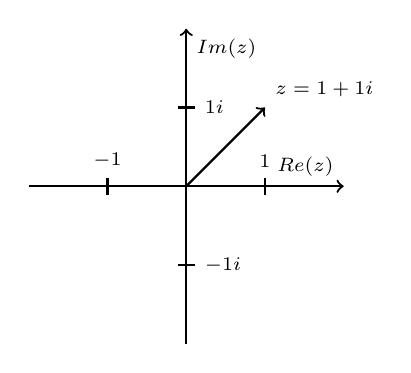
\begin{tikzpicture}
    \begin{scope}[thick,font=\scriptsize]
    % Axes:
    % Are simply drawn using line with the `->` option to make them arrows:
    % The main labels of the axes can be places using `node`s:
    \draw [->] (-2,0) -- (2,0) node [above left]  {$Re(z)$};
    \draw [->] (0,-2) -- (0,2) node [below right] {$Im(z)$};
    
    \draw (-1,-3pt) -- (-1,3pt)   node [above] {$-1$};
    \draw (1,-3pt) -- (1,3pt)   node [above] {$1$};
   \draw (-3pt,-1) -- (3pt,-1)   node [right] {$-1 i$};
   \draw (-3pt,1) -- (3pt,1)   node [right] {$1 i$};

%    \foreach \n in {-1,...,-1,2,1,...,1}{%
%        \draw (\n,-3pt) -- (\n,3pt)   node [above] {$\n$};
%        \draw (-3pt,\n) -- (3pt,\n)   node [right] {$\n i$};
%    }
    \draw [->] (0,0) -- (1,1) node [above right]{$z = 1 + 1i$};
    \end{scope}
	\end{tikzpicture}
	\caption{Complex Plane}
	\label{complex-plane}
	\end{wrapfigure}
	
	A complex number is also called a two-dimensional number because it has two parts: 
	
	\vspace{-15pt}
	the real part $Re(z) = a$, and the imaginary part $Re(z) = b$, 
	
	\vspace{-15pt}
	that can be plotted to a two-dimensional field (see \autoref{complex-plane}).
	In this work I will not explain the properties of complex numbers and we will therefore move on with 
	studying three-dimensional numbers.
	
	\vspace{15pt}
	
	There might be many ways of how to define three-dimensional numbers, but in this case we will focus the
	most on the property to invert the multiplication of two three-dimensional numbers.
	
	\newpage
	\section{Exploration}
	
To explore which properties are needed to have the most satisfying algebraic group of three-dimensional numbers, let's define a three-dimensional number as followed:

\begin{tcolorbox}[title=Percomplex Numbers,colframe=blue!60, colback=blue!5]
\begin{align*}
\mathfrak{p} &= a + bi + cp && a,b,c \in \mathbb{R} \hspace{3pt} \text{and} \hspace{3pt} i,p \hspace{3pt} \text{are undefined for now ...} \\
\mathfrak{p} &\in \mathfrak{P} 
\end{align*}
\end{tcolorbox}

The strucure $(\mathfrak{P}, +)$ is an infinate abelian group.
I will leave the proof open as it's trivial.
I will focus more on the strucuture $(\mathfrak{P}, \cdot)$ in the following.

Percomplex Multiplication is not necessarily closed.

\begin{align*}
\mathfrak{p}_1 \cdot \mathfrak{p}_2 = \hspace{3pt} & (x_1 + x_2i +x_3p) \cdot (y_1 + y_2i + y_3p)
&&& x_1,x_2,x_3, y_1,y_2,y_3 \in \mathbb{R} \\
= \hspace{3pt} & (x_1 \cdot y_1 + x_1 \cdot y_2i + x_1 \cdot y_3p) &+ \\
& (x_2i \cdot y_1 + x_2i \cdot y_2i + x_2i \cdot y_3p) &+ \\
& (x_3p \cdot y_1 + x_3p \cdot y_2i + x_3p \cdot x_3p)  \\
\end{align*}

It depends on how we define the multiplication of $i$ and $p$.

There are a few options that need to be viewed to keep any percomplex number $\mathfrak{p}$ three-dimensional

\begin{align*}
1) && i \cdot p &= i \\
2) && i \cdot p &= p \\
3) && i \cdot p &= n, & n \in \mathbb{R} \\
4) && i \cdot p &\neq p \cdot i
\end{align*}


An important property for such a group is to be invertible, which means
that each element $\mathfrak{p} \neq 0$ has an inverse $\frac{1}{\mathfrak{p}}$.

With complex number this can be solved by the \textit{complex conjugate} $\overline{z} = a - bi$,
as this can be used to create an inverse.

\begin{align*}
\frac{1}{z} &= \frac{1}{a + bi} \\
&= \frac{1}{a + bi} \cdot \frac{\overline{z}}{\overline{z}} \\
&= \frac{1}{a + bi} \cdot \frac{a - bi}{a - bi} \\
&= \frac{a - bi}{(a + bi) \cdot (a - bi)} \\
&= \frac{a - bi}{a^2 + b^2} \\
&= \frac{a}{a^2 + b^2} - \frac{b}{a^2 + b^2} \cdot i
\end{align*}

In other words this property depends on the crucial fact that $z \cdot \overline{z} = a^2 + b^2$ which is a real number.
Therefore I will spend my effort on finding a way to multiply two percomplex numbers to get a real number as well. 
\begin{align*}
\mathfrak{p}_1 \cdot \mathfrak{p}_2 &= (x_1 + x_2i +x_3p) \cdot (y_1 + y_2i + y_3p) && x_1,x_2,x_3, y_1,y_2,y_3 \in \mathbb{R} \\
&= x_1 \cdot y_1 + x_1 \cdot y_2i + \cdots + x_3p \cdot y_2i + x_3p \cdot x_3p  \\
&\stackrel{!}{=} n &&  n \in \mathbb{R}
\end{align*}

It makes sense to try the same approach as with complex numbers.
\begin{align*}
\mathfrak{p} \cdot \overline{\mathfrak{p}} = \hspace{3pt}& (x_1 + x_2i +x_3p) \cdot (x_1 - x_2i - x_3p) &&& x_1,x_2,x_3 \in \mathbb{R} \\
= \hspace{3pt} & (x_1 \cdot x_1 + x_1 \cdot x_2i + x_1 \cdot x_3p)  &+ \\
& (x_2i \cdot x_1 + x_2i \cdot x_2i + x_2i \cdot x_3p) &+ \\
& (x_3p \cdot x_1 + x_3p \cdot x_2i + x_3p \cdot x_3p)
\end{align*}

Obviously if we multiply two percomplex numbers, we will get the quantity $i \cdot p$ or $p \cdot i$ , which is outside of the set if we don't apply a rule for that to be inside the set as well.

However if we apply rules to make $i \cdot p$ or $p \cdot i$ a part of the set again

	
	\newpage
	\section{Literature}
	
%	\defbibfilter{penis}{
%  type=misc or
%  type=inproceedings
%  %  type=thesis or
%%  type=inbook or
%}
	
	\printbibliography[type=article, title={Articles}]
	\printbibliography[type=thesis, title={Papers}]
	\printbibliography[type=inbook, title={Book Excerpts}]
	\printbibliography[type=inproceedings, title={Inproceedings}]
	


\end{document}